% \documentclass[11pt]{article}
%DIF LATEXDIFF DIFFERENCE FILE
%DIF DEL supplemental_orig.tex   Mon May 30 19:46:36 2016
%DIF ADD supplemental_rev.tex    Fri Jun 17 22:32:52 2016
\documentclass[useAMS,usenatbib,referee]{biomweb}
% \usepackage{amssymb, amsthm, amsmath}
\usepackage{amssymb, amsmath}
\usepackage{bm}
\usepackage{graphicx}
% \usepackage[authoryear]{natbib}
\usepackage{bm}
\usepackage{verbatim}
\usepackage{lineno}
\usepackage{times}
\usepackage{soul}
\usepackage{color}
\usepackage{enumitem}
% \usepackage{enumerate}
\usepackage{setspace}
\usepackage{appendix}
% \usepackage{caption}
% \captionsetup[table]{name=Web Table}

% cross-referencing appendices
\usepackage{xr}
%DIF 23c23
%DIF < \externaldocument{skewt_orig}
%DIF -------
\externaldocument{skewt_rev} %DIF > 
%DIF -------

% \usepackage[left=1in,top=1in,right=1in]{geometry}
% \pdfpageheight 11in
% \pdfpagewidth 8.5in
% \linespread{2.0}
\newcommand{\btheta}{ \mbox{\boldmath $\theta$}}
\newcommand{\bmu}{ \mbox{\boldmath $\mu$}}
\newcommand{\balpha}{ \mbox{\boldmath $\alpha$}}
\newcommand{\bbeta}{ \mbox{\boldmath $\beta$}}
\newcommand{\bdelta}{ \mbox{\boldmath $\delta$}}
\newcommand{\blambda}{ \mbox{\boldmath $\lambda$}}
\newcommand{\bgamma}{ \mbox{\boldmath $\gamma$}}
\newcommand{\brho}{ \mbox{\boldmath $\rho$}}
\newcommand{\bpsi}{ \mbox{\boldmath $\psi$}}
\newcommand{\bepsilon}{ \mbox{\boldmath $\epsilon$}}
\newcommand{\bomega}{ \mbox{\boldmath $\omega$}}
\newcommand{\bOmega}{ \mbox{\boldmath $\Omega$}}
\newcommand{\bDelta}{ \mbox{\boldmath $\Delta$}}
\newcommand{\bSigma}{ \mbox{\boldmath $\Sigma$}}
\newcommand{\bPsi}{\mbox{\boldmath $\Psi$}}
\newcommand{\bOne}{\mbox{\boldmath $1$}}
\newcommand{\omu}{\overline{\mu}}
\newcommand{\oSigma}{\overline{\Sigma}}
\newcommand{\Yt}{{\tilde Y}}
\newcommand{\bA}{ \mbox{\bf A}}
\newcommand{\bP}{ \mbox{\bf P}}
\newcommand{\bx}{ \mbox{\bf x}}
\newcommand{\bX}{ \mbox{\bf X}}
\newcommand{\bB}{ \mbox{\bf B}}
\newcommand{\bZ}{ \mbox{\bf Z}}
\newcommand{\by}{ \mbox{\bf y}}
\newcommand{\bY}{ \mbox{\bf Y}}
\newcommand{\bz}{ \mbox{\bf z}}
\newcommand{\bh}{ \mbox{\bf h}}
\newcommand{\br}{ \mbox{\bf r}}
\newcommand{\bt}{ \mbox{\bf t}}
\newcommand{\bs}{ \mbox{\bf s}}
\newcommand{\bb}{ \mbox{\bf b}}
\newcommand{\bL}{ \mbox{\bf L}}
\newcommand{\bu}{ \mbox{\bf u}}
\newcommand{\bv}{ \mbox{\bf v}}
\newcommand{\bV}{ \mbox{\bf V}}
\newcommand{\bW}{ \mbox{\bf W}}
\newcommand{\bG}{ \mbox{\bf G}}
\newcommand{\bH}{ \mbox{\bf H}}
\newcommand{\bw}{ \mbox{\bf w}}
\newcommand{\bo}{ \mbox{\bf o}}
\newcommand{\bfe}{ \mbox{\bf e}}
\newcommand{\iid}{\stackrel{iid}{\sim}}
\newcommand{\indep}{\stackrel{indep}{\sim}}
\newcommand{\calR}{{\cal R}}
\newcommand{\calG}{{\cal G}}
\newcommand{\calD}{{\cal D}}
\newcommand{\calS}{{\cal S}}
\newcommand{\calB}{{\cal B}}
\newcommand{\calA}{{\cal A}}
\newcommand{\calT}{{\cal T}}
\newcommand{\calO}{{\cal O}}
\newcommand{\argmax}{{\mathop{\rm arg\, max}}}
\newcommand{\argmin}{{\mathop{\rm arg\, min}}}
\newcommand{\Frechet}{\mbox{Fr$\acute{\mbox{e}}$chet }}
\newcommand{\Matern}{\mbox{Mat$\acute{\mbox{e}}$rn }}
\newcommand{\ballunion}{B_a(\bs_1) \cup B_b(\bs_2) }

\newcommand{\beq}{ \begin{equation}}
\newcommand{\eeq}{ \end{equation}}
\newcommand{\beqn}{ \begin{eqnarray}}
\newcommand{\eeqn}{ \end{eqnarray}}
%DIF 30a30
\renewcommand{\fref}[1]{Web Figure~\ref{#1}} %DIF > 
%DIF -------

\title[Web-based Supplementary Materials for A Space-time Skew-$t$ Model for Threshold Exceedances]{Web-based Supplementary Materials for A Space-time Skew-$t$ Model for Threshold Exceedances by Morris, Reich, Thibaud, and Cooley}
\author
{Samuel A Morris$^{1,*}$\email{samorris@ncsu.edu},
Brian J Reich$^{1}$,
Emeric Thibaud$^{2}$, and
Daniel Cooley$^{2}$\\
$^{1}$Department of Statistics, North Carolina State University, Raleigh, North Carolina, U.S.A. \\
$^{2}$Department of Statistics, Colorado State University, Fort Collins, Colorado, U.S.A.}
%DIF PREAMBLE EXTENSION ADDED BY LATEXDIFF
%DIF UNDERLINE PREAMBLE %DIF PREAMBLE
\RequirePackage[normalem]{ulem} %DIF PREAMBLE
\RequirePackage{color}\definecolor{RED}{rgb}{1,0,0}\definecolor{BLUE}{rgb}{0,0,1} %DIF PREAMBLE
\providecommand{\DIFadd}[1]{{\protect\color{blue}\uwave{#1}}} %DIF PREAMBLE
\providecommand{\DIFdel}[1]{{\protect\color{red}\sout{#1}}}                      %DIF PREAMBLE
%DIF SAFE PREAMBLE %DIF PREAMBLE
\providecommand{\DIFaddbegin}{} %DIF PREAMBLE
\providecommand{\DIFaddend}{} %DIF PREAMBLE
\providecommand{\DIFdelbegin}{} %DIF PREAMBLE
\providecommand{\DIFdelend}{} %DIF PREAMBLE
%DIF FLOATSAFE PREAMBLE %DIF PREAMBLE
\providecommand{\DIFaddFL}[1]{\DIFadd{#1}} %DIF PREAMBLE
\providecommand{\DIFdelFL}[1]{\DIFdel{#1}} %DIF PREAMBLE
\providecommand{\DIFaddbeginFL}{} %DIF PREAMBLE
\providecommand{\DIFaddendFL}{} %DIF PREAMBLE
\providecommand{\DIFdelbeginFL}{} %DIF PREAMBLE
\providecommand{\DIFdelendFL}{} %DIF PREAMBLE
%DIF END PREAMBLE EXTENSION ADDED BY LATEXDIFF

\begin{document} %\linenumbers
\maketitle
% \begin{center}
% {\Large {\bf Supplemental material for A space-time skew-$t$ model for threshold exceedances}}\\

% {\large Samuel A Morris\footnote[1]{North Carolina State University}, Brian J Reich\footnotemark[1]{}, Emeric Thibaud\footnote[2]{Colorado State University}, and Daniel Cooley\footnotemark[2]{}}

% \today
% \end{center}

% \appendix
\DIFdelbegin %DIFDELCMD < \renewcommand{\thesection}{Web Appendix \Alph{section}}
%DIFDELCMD < %%%
\DIFdelend \DIFaddbegin \renewcommand{\thesection}{Web Appendix~\Alph{section}}
\DIFaddend % \renewcommand{\tablename}{Web Table}
% \renewcommand{\figurename}{Web Figure}
% \renewcommand{\thetable}{Web Table \arabic{table}}

\section{MCMC details} \DIFdelbegin %DIFDELCMD < %DIFDELCMD < \label{a:mcmc}%%%
%DIFDELCMD < %%%
\DIFdelend \DIFaddbegin \label{sta:mcmc}
\DIFaddend The MCMC sampling for the model \DIFdelbegin \DIFdel{\ref{s:hier} }\DIFdelend \DIFaddbegin \DIFadd{in }\sref{sts:hier} \DIFaddend is done using {\tt R} (http://www.r-project.org). Whenever possible, we select conjugate priors (see \DIFdelbegin \DIFdel{Appendix \ref{a:posterior}}\DIFdelend \DIFaddbegin \aref{sta:posterior}\DIFaddend ); however, for some of the parameters, no conjugate prior distributions exist.
For these parameters, we use a random walk Metropolis-Hastings update step.
In each Metropolis-Hastings update, we tune the algorithm during the burn-in period to give acceptance rates near 0.40.

\subsection*{Spatial knot locations}
For each day, we update the spatial knot locations, $\bw_1, \ldots, \bw_K$, using a Metropolis-Hastings block update.
Because the spatial domain is bounded, we generate candidate knots using the transformed knots $\bw^*_1, \ldots, \bw^*_K$ (see \DIFdelbegin \DIFdel{section \ref{s:temporal}}\DIFdelend \DIFaddbegin \sref{sts:temporal}\DIFaddend ) and a random walk bivariate Gaussian candidate distribution
\begin{align*}
	{\bw^*_k}^{(c)} \sim \text{N}({\bw^*_k}^{(r - 1)}, s^2 I_2)
\end{align*}
where ${\bw^*_k}^{(r - 1)}$ is the location for the transformed knot at MCMC iteration $r - 1$, $s$ is a tuning parameter, and $I_2$ is an identity matrix.
\DIFaddbegin \DIFadd{Let $\bY_t = [Y(\bs_1), \ldots, Y(\bs_n)]$ be the vector of observed responses at each site for day $t$.
}\DIFaddend After candidates have been generated for all $K$ knots, the acceptance ratio is
\begin{align*}
  R = \left\{ \DIFdelbegin \DIFdel{\frac{ l[ Y_t(\bs | \bw_1^{(c)}, \ldots, \bw_K^{(c)}, \ldots)] }{l[ Y_t(\bs | \bw_1^{(r - 1)}, \ldots, \bw_K^{(r - 1)}, \ldots)]} }\DIFdelend \DIFaddbegin \DIFadd{\frac{ l[ \bY_t | \bw_1^{(c)}, \ldots, \bw_K^{(c)}, \ldots] }{l[ \bY_t | \bw_1^{(r - 1)}, \ldots, \bw_K^{(r - 1)}, \ldots]} }\DIFaddend \right\} \times \left\{ \frac{ \prod_{k = 1}^{K}\phi(\bw_k^{(c)})}{ \prod_{k = 1}^{K}\phi(\bw_k^{(r - 1)})} \right\} \times \left\{ \frac{ \prod_{k = 1}^{K} p({\bw^*_k}^{(c)})}{ \prod_{k = 1}^{K} p({\bw^*_k}^{(r - 1)})}\right\}
\end{align*}
where $l$ is the likelihood given in \DIFdelbegin \DIFdel{(\ref{eq:hier})}\DIFdelend \DIFaddbegin \eref{steq:hier}\DIFaddend , and $p(\cdot)$ is the prior either taken from the time series \DIFdelbegin \DIFdel{given in (\ref{s:temporal}}\DIFdelend \DIFaddbegin \DIFadd{(see }\sref{sts:temporal}\DIFaddend ) or assumed to be uniform over $\calD$.
The candidate knots are accepted with probability $\min\{R, 1\}$.

\subsection*{Spatial random effects}
If there is no temporal dependence amongst the observations, we use a Gibbs update for $z_{tk}$, and the posterior distribution is given in \DIFdelbegin \DIFdel{\ref{a:posterior}}\DIFdelend \DIFaddbegin \aref{sta:posterior}\DIFaddend .
If there is temporal dependence amongst the observations, then we update $z_{tk}$ using a Metropolis-Hastings update.
Because this model uses $|z_{tk}|$, we generate candidate random effects using the $z^*_{tk}$ (see \DIFdelbegin \DIFdel{Section \ref{s:temporal}}\DIFdelend \DIFaddbegin \sref{sts:temporal}\DIFaddend ) and a random walk Gaussian candidate distribution
\begin{align*}
  {z^*_{tk}}^{(c)} \sim \text{N}({z^*_{tk}}^{(r - 1)}, s^2)
\end{align*}
where ${z^*_{tk}}^{(r-1)}$ is the value at MCMC iteration $r - 1$, and $s$ is a tuning parameter.
The acceptance ratio is
\begin{align*}
  R = \left\{ \DIFdelbegin \DIFdel{\frac{ l[Y_t(\bs) | z_{tk}^{(c)}, \ldots] }{ l[Y_t(\bs) | z_{tk}^{(r - 1)}]} }\DIFdelend \DIFaddbegin \DIFadd{\frac{ l[\bY_t | z_{tk}^{(c)}, \ldots] }{ l[\bY_t | z_{tk}^{(r - 1)}]} }\DIFaddend \right\} \times \left\{ \frac{ p[ z_{tk}^{(c)} ] }{ p[ z_{tk}^{(r - 1)}]}\right\}
\end{align*}
where $p[\cdot]$ is the prior taken from the time series given in \DIFdelbegin \DIFdel{Section \ref{s:temporal}}\DIFdelend \DIFaddbegin \sref{sts:temporal}\DIFaddend .
The candidate is accepted with probability $\min\{R, 1\}$.

\subsection*{Variance terms}
When there is more than one site in a partition, then we update $\sigma^2_{tk}$ using a Metropolis-Hastings update.
First, we generate a candidate for $\sigma^2_{tk}$ using an IG$(a^*/s, b^*/s)$ candidate distribution in an independence Metropolis-Hastings update where $a^* = (n_{tk} + 1) / 2 + a$, \DIFdelbegin \DIFdel{$b^* = [Y_{tk}^T \Sigma^{-1}_{tk} Y_{tk} + z_{tk}^2] / 2 + b$}\DIFdelend \DIFaddbegin \DIFadd{$b^* = [\bY_{tk}^\top \Sigma^{-1}_{tk} \bY_{tk} + z_{tk}^2] / 2 + b$}\DIFaddend , $n_{tk}$ is the number of sites in partition $k$ on day $t$, and \DIFdelbegin \DIFdel{$Y_{tk}$ }\DIFdelend \DIFaddbegin \DIFadd{$\bY_{tk}$ }\DIFaddend and $\Sigma^{-1}_{tk}$ are the observations and precision matrix for partition $k$ on day $t$.
The acceptance ratio is
\begin{align*}
  R = \left\{
    \DIFdelbegin \DIFdel{\frac{ l[Y_t(\bs) | {\sigma^2_{tk}}^{(c)}, \ldots] }{ l[Y_t(\bs) | {\sigma^2_{tk}}^{(r - 1)}]}
    }\DIFdelend \DIFaddbegin \DIFadd{\frac{ l[\bY_t | {\sigma^2_{tk}}^{(c)}, \ldots] }{ l[\bY_t | {\sigma^2_{tk}}^{(r - 1)}]}
    }\DIFaddend \right\} \times \left\{
    \frac{ l[z_{tk} | {\sigma^2_{tk}}^{(c)}, \ldots] }{ l[z_{tk} | {\sigma^2_{tk}}^{(r - 1)}, \ldots] }
    \right\} \times \left\{
    \frac{ p[ {\sigma^2_{tk}}^{(c)} ] }{ p[ {\sigma^2_{tk}}^{(r - 1)}] }
    \right\} \times \left\{
    \frac{ c[ {\sigma^2_{tk}}^{(r - 1)}] }{ c[ {\sigma^2_{tk}}^{(c)}]}
    \right\}
\end{align*}
where $p[\cdot]$ is the prior either taken from the time series given in \DIFdelbegin \DIFdel{Section \ref{s:temporal} }\DIFdelend \DIFaddbegin \sref{sts:temporal} \DIFaddend or assumed to be IG$(a, b)$, and $c[\cdot]$ is the candidate distribution.
The candidate is accepted with probability $\min\{R, 1\}$.

\subsection*{Spatial covariance parameters}
We update the three spatial covariance parameters, $\log(\rho)$, $\log(\nu)$, $\gamma$, using a Metropolis-Hastings block update step.
First, we generate a candidate using a random walk Gaussian candidate distribution
\begin{align*}
	\log(\rho)^{(c)} \sim \text{N}(\log(\rho)^{(r - 1)}, s^2)
\end{align*}
where $\log(\rho)^{(r-1)}$ is the value at MCMC iteration $r - 1$, and $s$ is a tuning parameter.
Candidates are generated for $\log(\nu)$ and $\gamma$ in a similar fashion.
The acceptance ratio is
\begin{align*}
	R = \left\{ \DIFdelbegin \DIFdel{\frac{ \prod_{t = 1}^{T} l[Y_t(\bs) | \rho^{(c)}, \nu^{(c)}, \gamma^{(c)}, \ldots] }{\prod_{t = 1}^{T} l[Y_t(\bs) | \rho^{(r-1)}, \nu^{(r-1)}, \gamma^{(r-1)}, \ldots] } }\DIFdelend \DIFaddbegin \DIFadd{\frac{ \prod_{t = 1}^{n_t} l[Y_t(\bs) | \rho^{(c)}, \nu^{(c)}, \gamma^{(c)}, \ldots] }{\prod_{t = 1}^{n_t} l[Y_t(\bs) | \rho^{(r-1)}, \nu^{(r-1)}, \gamma^{(r-1)}, \ldots] } }\DIFaddend \right\} \times \left\{ \frac{ p[\rho^{(c)}] }{ p[\rho^{(r - 1)] } } \right\} \times \left\{ \frac{ p[\nu^{(c)}] }{ p[\nu^{(r - 1)}] } \right\} \times \left\{ \frac{ p[ \gamma^{(c)} ] }{ p[\gamma^{(r - 1)} ] } \right\}.
\end{align*}
All three candidates are accepted with probability $\min\{R, 1\}$.

\section{Posterior distributions} \DIFdelbegin %DIFDELCMD < %DIFDELCMD < \label{a:posterior}%%%
%DIFDELCMD < %%%
\DIFdelend \DIFaddbegin \label{sta:posterior}
\DIFaddend 

\subsection*{Conditional posterior of $z_{tk} \mid \ldots $}\DIFdelbegin %DIFDELCMD < %DIFDELCMD < \label{s:mvcondu}%%%
%DIFDELCMD < %%%
\DIFdelend \DIFaddbegin \label{sts:mvcondu}
\DIFaddend If knots are independent over days, then the conditional posterior distribution of $|z_{tk}|$ is conjugate.
For simplicity, drop the subscript $t$, let \DIFdelbegin \DIFdel{$\tilde{z}_{tk} = |z_{tk}|$, }\DIFdelend \DIFaddbegin \DIFadd{$\tilde{z}_{k} = |z_{k}|$, $\tilde{\bz}_{k^c}$ be the vector of $[|z(\bs_1)|, \ldots, |z(\bs_n)|]$ for $\bs \notin P_k$, $\bX = [\bX(\bs_1), \ldots, \bX(\bs_n)]^\top$, let $\bY_k$ and $\bX_k$ be the observations and covariate measurements for $\bs \in P_k$, and let $\bY_{k^c}$ }\DIFaddend and \DIFdelbegin \DIFdel{define
}\DIFdelend \DIFaddbegin \DIFadd{$\bX_{k^c}$ be the observations and covariate measurements for $\bs \notin P_k$ and define
}\DIFaddend \begin{align*}
\DIFdelbegin \DIFdel{R(}%DIFDELCMD < \bs%%%
\DIFdel{) }\DIFdelend \DIFaddbegin \bR \DIFaddend = \left\{
    \DIFdelbegin %DIFDELCMD < \begin{array}{ll}
%DIFDELCMD <         Y(\bs) - X(\bs) \beta &s \in P_l\\[1em]
%DIFDELCMD <         Y(\bs) - X(\bs) \beta - \lambda \tilde{z}(\bs) \qquad & s \notin P_l
%DIFDELCMD <     \end{array}
%DIFDELCMD < %%%
\DIFdelend \DIFaddbegin \begin{array}{ll}
        \bY_k - \bX_k \bbeta & \bs \in P_k\\[1em]
        \bY_{k^c} - \bX_{k^c} \bbeta - \lambda \tilde{\bz}_{k^c} \qquad & \bs \notin P_k
    \end{array}
\DIFaddend \right.
\end{align*}
Let
\begin{align*}
    \DIFdelbegin \DIFdel{R}\DIFdelend \DIFaddbegin \bR\DIFaddend _1 &= \text{the vector of } \DIFdelbegin \DIFdel{R(}%DIFDELCMD < \bs%%%
\DIFdel{) }\DIFdelend \DIFaddbegin \bR \DIFaddend \text{ for } \DIFdelbegin \DIFdel{s }\DIFdelend \DIFaddbegin \bs \DIFaddend \in P\DIFdelbegin \DIFdel{_l }\DIFdelend \DIFaddbegin \DIFadd{_k }\DIFaddend \\
    \DIFdelbegin \DIFdel{R}\DIFdelend \DIFaddbegin \bR\DIFaddend _2 &= \text{the vector of } \DIFdelbegin \DIFdel{R(}%DIFDELCMD < \bs%%%
\DIFdel{) }\DIFdelend \DIFaddbegin \bR \DIFaddend \text{ for } \DIFdelbegin \DIFdel{s }\DIFdelend \DIFaddbegin \bs \DIFaddend \notin P\DIFdelbegin \DIFdel{_l }\DIFdelend \DIFaddbegin \DIFadd{_k }\DIFaddend \\
    \Omega &= \Sigma^{-1}.
\end{align*}
Then
\begin{align*}
    \pi(z\DIFdelbegin \DIFdel{_l }\DIFdelend \DIFaddbegin \DIFadd{_k }\DIFaddend | \ldots) &\propto \exp \left\{ -\frac{ 1 }{ 2 } \left[
        \left( \DIFdelbegin %DIFDELCMD < \begin{array}{c}
%DIFDELCMD <             R_1 - \lambda \tilde{z}_l \bOne\\
%DIFDELCMD <             R_2
%DIFDELCMD <         \end{array} %%%
\DIFdelend \DIFaddbegin \begin{array}{c}
            \bR_1 - \lambda \tilde{z}_k \bOne\\
            \bR_2
        \end{array} \DIFaddend \right)\DIFdelbegin \DIFdel{^T
        }\DIFdelend \DIFaddbegin \DIFadd{^\top
        }\DIFaddend \left( \begin{array}{cc}
            \Omega_{11} & \Omega_{12}\\
            \Omega_{21} & \Omega_{22}
        \end{array} \right)
        \left( \DIFdelbegin %DIFDELCMD < \begin{array}{c}
%DIFDELCMD <             R_1 - \lambda \tilde{z}_l \bOne\\
%DIFDELCMD <             R_2
%DIFDELCMD <         \end{array} %%%
\DIFdelend \DIFaddbegin \begin{array}{c}
            \bR_1 - \lambda \tilde{z}_k \bOne\\
            \bR_2
        \end{array} \DIFaddend \right)
        +  \DIFdelbegin \DIFdel{\frac{ {\tilde{z}_l}^2 }{ \sigma_l^2 }}\DIFdelend \DIFaddbegin \DIFadd{\frac{ {\tilde{z}_k}^2 }{ \sigma_k^2 }}\DIFaddend \right]
    \right\} I(z\DIFdelbegin \DIFdel{_l }\DIFdelend \DIFaddbegin \DIFadd{_k }\DIFaddend > 0) \\
        &\propto \exp \left\{ -\frac{ 1 }{ 2 } \left[ \Lambda\DIFdelbegin \DIFdel{_l }\DIFdelend \DIFaddbegin \DIFadd{_k }\DIFaddend {\tilde{z}\DIFdelbegin \DIFdel{_l}\DIFdelend \DIFaddbegin \DIFadd{_k}\DIFaddend }^2 - 2 \mu\DIFdelbegin \DIFdel{_l }\DIFdelend \DIFaddbegin \DIFadd{_k }\DIFaddend \tilde{z}\DIFdelbegin \DIFdel{_l }\DIFdelend \DIFaddbegin \DIFadd{_k }\DIFaddend \right] \right\}
\end{align*}
where
\begin{align*}
    \mu\DIFdelbegin \DIFdel{_l }\DIFdelend \DIFaddbegin \DIFadd{_k }\DIFaddend &= \lambda ( \DIFdelbegin \DIFdel{R}\DIFdelend \DIFaddbegin \bR\DIFaddend _1\DIFdelbegin \DIFdel{^T }\DIFdelend \DIFaddbegin \DIFadd{^\top }\DIFaddend \Omega_{11} + \DIFdelbegin \DIFdel{R}\DIFdelend \DIFaddbegin \bR\DIFaddend _2\DIFdelbegin \DIFdel{^T }\DIFdelend \DIFaddbegin \DIFadd{^\top }\DIFaddend \Omega_{21} )\bOne\\
    \Lambda\DIFdelbegin \DIFdel{_l }\DIFdelend \DIFaddbegin \DIFadd{_k }\DIFaddend &= \lambda^2 \bOne\DIFdelbegin \DIFdel{^T }\DIFdelend \DIFaddbegin \DIFadd{^\top }\DIFaddend \Omega_{11} \bOne + \DIFdelbegin \DIFdel{\frac{ 1 }{ \sigma^2_l }}\DIFdelend \DIFaddbegin \DIFadd{\frac{ 1 }{ \sigma^2_k }}\DIFaddend .
\end{align*}
Then \DIFdelbegin \DIFdel{$\tilde{Z}_l | \ldots \sim N_{(0, \infty)} (\Lambda_l^{-1} \mu_l, \Lambda_l^{-1})$
}\DIFdelend \DIFaddbegin \DIFadd{$\tilde{z}_k | \ldots \sim N_{(0, \infty)} (\Lambda_k^{-1} \mu_k, \Lambda_k^{-1})$
}\DIFaddend 

\subsection*{Conditional posterior of \DIFdelbegin \DIFdel{$\beta \mid \ldots$}\DIFdelend \DIFaddbegin \DIFadd{$\bbeta, \lambda \mid \ldots$}\DIFaddend }\DIFdelbegin %DIFDELCMD < %DIFDELCMD < \label{s:betapost}%%%
%DIFDELCMD < %%%
\DIFdel{Let $\beta \sim \mbox{N}_{p}(0, \Lambda_0)$ }\DIFdelend \DIFaddbegin \label{sts:betapost}
\DIFadd{For models that do not include a skewness parameter, we update $\bbeta$ as follows.
Let $\bbeta \sim \mbox{N}_{p}(0, \Lambda_0)$ }\DIFaddend where $\Lambda_0$ is a precision matrix.
Then
\begin{align*}
    \pi(\DIFdelbegin \DIFdel{\beta }\DIFdelend \DIFaddbegin \bbeta \DIFaddend \mid \ldots) & \propto \exp \left\{ - \frac{ 1 }{ 2 } \DIFdelbegin \DIFdel{\beta^T }\DIFdelend \DIFaddbegin \bbeta\DIFadd{^\top }\DIFaddend \Lambda_0 \DIFdelbegin \DIFdel{\beta }\DIFdelend \DIFaddbegin \bbeta \DIFaddend - \frac{ 1 }{ 2 } \sum\DIFdelbegin \DIFdel{_{t = 1 }^T }\DIFdelend \DIFaddbegin \DIFadd{_{t = 1}^{n_t} }\DIFaddend [\bY_t -\DIFdelbegin \DIFdel{X}\DIFdelend \DIFaddbegin \bX\DIFaddend _t \DIFdelbegin \DIFdel{\beta - \lambda |z_t|}\DIFdelend \DIFaddbegin \bbeta\DIFaddend ]\DIFdelbegin \DIFdel{^T }\DIFdelend \DIFaddbegin \DIFadd{^\top }\DIFaddend \Omega [\bY_t - \DIFdelbegin \DIFdel{X}\DIFdelend \DIFaddbegin \bX\DIFaddend _t \DIFdelbegin \DIFdel{\beta - \lambda |z_t|}\DIFdelend \DIFaddbegin \bbeta\DIFaddend ] \right\} \\
     & \propto \exp \left\{ -\frac{ 1 }{ 2 } \left[ \DIFdelbegin \DIFdel{\beta^T }\DIFdelend \DIFaddbegin \bbeta\DIFadd{^\top }\DIFaddend \Lambda_\beta \DIFdelbegin \DIFdel{\beta  }\DIFdelend \DIFaddbegin \bbeta  \DIFaddend - 2 \sum\DIFdelbegin \DIFdel{_{ t = 1 }^T }%DIFDELCMD < [ %%%
\DIFdel{\beta^T X}\DIFdelend \DIFaddbegin \DIFadd{_{t = 1}^{n_t} (}\bbeta\DIFadd{^\top }\bX\DIFaddend _t\DIFdelbegin \DIFdel{^T }\DIFdelend \DIFaddbegin \DIFadd{^\top }\DIFaddend \Omega \DIFdelbegin \DIFdel{(}\DIFdelend \bY_t\DIFdelbegin \DIFdel{- \lambda |z_t| }\DIFdelend ) \DIFdelbegin %DIFDELCMD < ] %%%
\DIFdelend \right] \right\} \\
     & \propto \mbox{N} ( \Lambda_\beta^{-1} \mu_\beta , \Lambda_\beta^{-1})
\end{align*}
where
\begin{align*}
    \mu_\beta &= \sum\DIFdelbegin \DIFdel{_{t=1}^{T} }%DIFDELCMD < \left[ %%%
\DIFdel{X}\DIFdelend \DIFaddbegin \DIFadd{_{t = 1}^{n_t} }\bX\DIFaddend _t\DIFdelbegin \DIFdel{^T }\DIFdelend \DIFaddbegin \DIFadd{^\top }\DIFaddend \Omega \DIFdelbegin \DIFdel{(}\DIFdelend \bY_t \DIFdelbegin \DIFdel{- \lambda |z_t|) }%DIFDELCMD < \right]%%%
\DIFdelend \\
    \Lambda_\beta &= \Lambda_0 + \sum\DIFdelbegin \DIFdel{_{ t = 1 }^{ T} X}\DIFdelend \DIFaddbegin \DIFadd{_{t = 1}^{n_t} }\bX\DIFaddend _t\DIFdelbegin \DIFdel{^T }\DIFdelend \DIFaddbegin \DIFadd{^\top }\DIFaddend \Omega \DIFdelbegin \DIFdel{X}\DIFdelend \DIFaddbegin \bX\DIFaddend _t.
\end{align*}
\DIFaddbegin \DIFadd{For models that do include a skewness parameter, a simple augmentation of the covariate matrix $\bX$ and parameter vector $\bbeta$ allows for a block update of both $\bbeta$ and $\lambda$.
Let $\bX^*_{t} = [\bX_t, |\bz_{t}|]$ where $\bz_t = [z(\bs_1), \ldots, z(\bs_{n})]^\top$ and let $\bbeta^* = (\beta_1, \ldots, \beta_p, \lambda)^\top$.
So to incorporate the $N(0, \sigma^2_\lambda)$ prior on $\lambda$, let $\bbeta^* \sim \mbox{N}_{p+1}(0, \Lambda^*_0)$ where
}\begin{align*}
  \DIFadd{\Lambda^*_0 = \left( \begin{array}{cc}
    \Lambda_0 & 0 \\
    0         & \sigma^{-2}_\lambda
  \end{array}\right).
}\end{align*}
\DIFadd{Then the update for both $\bbeta$ and $\lambda$ is done using the conjugate prior given above with $\bX_t = \bX_t^*$ and $\bbeta = \bbeta^*$
}\DIFaddend 

\subsection*{Conditional posterior of $\sigma^2 \mid \ldots$}\DIFdelbegin %DIFDELCMD < %DIFDELCMD < \label{s:sigpost}%%%
%DIFDELCMD < %%%
\DIFdelend \DIFaddbegin \label{sts:sigpost}
\DIFaddend In the case where $L = 1$ and temporal dependence is negligible, then $\sigma^2$ has a conjugate posterior distribution.
Let \DIFdelbegin \DIFdel{$\sigma_t^2 \iid \mbox{IG}(\alpha_0, \beta_0)$}\DIFdelend \DIFaddbegin \DIFadd{$\sigma_t^2 \iid \mbox{IG}(\alpha_0 / 2, \beta_0 / 2)$}\DIFaddend . For simplicity, drop the subscript $t$. Then
\begin{align*}
    \pi(\sigma^2 \mid \ldots) & \propto (\sigma^2)\DIFdelbegin \DIFdel{^{ -\alpha_0 - 1 / 2 - n / 2 - 1} }\DIFdelend \DIFaddbegin \DIFadd{^{ -\alpha_0 / 2 - 1 / 2 - n / 2 - 1} }\DIFaddend \exp \left\{ -\DIFdelbegin \DIFdel{\frac{\beta_0}{\sigma^2} }\DIFdelend \DIFaddbegin \DIFadd{\frac{\beta_0}{2\sigma^2} }\DIFaddend - \frac{ |z|^2 }{2 \sigma^2} - \DIFdelbegin \DIFdel{\frac{ (\bY - \bmu)^T \Sigma^{-1} (\bY - \bmu) }{2 \sigma^2} }\DIFdelend \DIFaddbegin \DIFadd{\frac{ (\bY - \bmu)^\top \Sigma^{-1} (\bY - \bmu) }{2 \sigma^2} }\DIFaddend \right\} \\
    & \propto (\sigma^2)\DIFdelbegin \DIFdel{^{ -\alpha_0 - 1 / 2 - n / 2 - 1} }\DIFdelend \DIFaddbegin \DIFadd{^{ -(\alpha_0 - 1 - n) / 2 - 1} }\DIFaddend \exp \left\{ - \DIFdelbegin \DIFdel{\frac{ 1 }{ \sigma^2 } }\DIFdelend \DIFaddbegin \DIFadd{\frac{ 1 }{ 2 \sigma^2 } }\DIFaddend \left[\beta_0 + \DIFdelbegin \DIFdel{\frac{ |z|^2 }{ 2 } }\DIFdelend \DIFaddbegin \DIFadd{|z|^2 }\DIFaddend + \DIFdelbegin \DIFdel{\frac{ 1 }{ 2 } }\DIFdelend (\bY - \bmu)\DIFdelbegin \DIFdel{^T }\DIFdelend \DIFaddbegin \DIFadd{^\top }\DIFaddend \Sigma^{-1} (\bY - \DIFdelbegin \DIFdel{\mu}\DIFdelend \DIFaddbegin \bmu\DIFaddend ) \right] \right\} \\
    & \propto \mbox{IG} (\alpha^*, \beta^*)
\end{align*}
where
\begin{align*}
    \alpha^* &= \DIFdelbegin \DIFdel{\alpha_0 + \frac{1}{2} + \frac{n}{2} }\DIFdelend \DIFaddbegin \DIFadd{\frac{\alpha_0 + 1 + n}{2} }\DIFaddend \\
    \beta^* &= \DIFaddbegin \DIFadd{\frac{1}{2} }\left[ \DIFaddend \beta_0 + \DIFdelbegin \DIFdel{\frac{ |z|^2 }{ 2 } }\DIFdelend \DIFaddbegin \DIFadd{|z|^2 }\DIFaddend + \DIFdelbegin \DIFdel{\frac{ 1 }{ 2 }}\DIFdelend (\bY - \bmu)\DIFdelbegin \DIFdel{^T }\DIFdelend \DIFaddbegin \DIFadd{^\top }\DIFaddend \Sigma^{-1} (\bY - \bmu) \DIFaddbegin \right]\DIFaddend .
\end{align*}
In the case that \DIFdelbegin \DIFdel{$L > 1$}\DIFdelend \DIFaddbegin \DIFadd{$K > 1$}\DIFaddend , a random walk Metropolis Hastings step will be used to update \DIFdelbegin \DIFdel{$\sigma^2_{lt}$}\DIFdelend \DIFaddbegin \DIFadd{$\sigma^2_{kt}$}\DIFaddend .

\DIFdelbegin \subsection*{\DIFdel{Conditional posterior of $\lambda \mid \ldots$}}%DIFAUXCMD
%DIFDELCMD < %DIFDELCMD < \label{s:lambdapost}%%%
%DIFDELCMD < %%%
\DIFdel{For convergence purposes we model $\lambda = \lambda_1 \lambda_2$ where
}\begin{eqnarray*}
  \DIFdel{\lambda_1 }&\DIFdel{= \left\{ \begin{array}{ll}
      +1 \quad & \text{w.p.} 0.5\\
      -1 \quad & \text{w.p.} 0.5
   \end{array}\right.}\\
   \DIFdel{\lambda^2_2 }& \DIFdel{\sim IG(\alpha_\lambda, \beta_\lambda).}\\
\end{eqnarray*}
%DIFAUXCMD
\DIFdel{Then
}\begin{eqnarray*}
  \DIFdel{\pi(\lambda_2 \mid \ldots) }&\DIFdel{\propto }{\DIFdel{\lambda_2^2}}\DIFdel{^{(-\alpha_\lambda - 1)} \exp\left\{ - \frac{ \beta_\lambda }{ \lambda_2^2} \right\} \prod_{t = 1}^{T} \prod_{k = 1}^K \frac{1} }{\DIFdel{\lambda_2}} \DIFdel{\exp\left\{ - \frac{ z^2_{tk} }{ 2 \lambda_2^2  \sigma_{tk})^2} \right\} }\\
   & \DIFdel{\propto }{\DIFdel{\lambda_2^2}}\DIFdel{^{(-\alpha_\lambda - kt - 1)} \exp \left\{ -\frac{1}{\lambda^2_2} \left[ \beta_\lambda + \frac{ z^2 }{2 \sigma^2_{tk}} \right] \right\}
}\end{eqnarray*}
%DIFAUXCMD
\DIFdel{Then $\lambda_2 \mid \ldots \sim IG \left(\alpha_\lambda + kt, \beta_\lambda + \frac{ z^2 }{2 \sigma^2_{tk}} \right)$
}%DIFDELCMD < 

%DIFDELCMD < %%%
\DIFdelend \section{Proof that $\lim_{h \rightarrow \infty} \pi(h) = 0$} \DIFdelbegin %DIFDELCMD < %DIFDELCMD < \label{a:proofsamepartition}%%%
%DIFDELCMD < %%%
\DIFdelend \DIFaddbegin \label{sta:proofsamepartition}
\DIFadd{Let $c$ be the midpoint of $\bs_1$ and $\bs_2$.
Define $A$ as the circle centered at $c$ with radius $h / 2$ where $h = ||\bs_1 - \bs_2||$ is the distance between sites $\bs_1$ and $\bs_2$.
}\DIFaddend Consider a homogeneous spatial Poisson process \DIFdelbegin \DIFdel{with intensity $\mu$.
Define }\DIFdelend \DIFaddbegin \DIFadd{over $A$ with intensity given by
}\begin{align*}
  \DIFadd{\mu_{PP}(A) = \lambda_{PP} |A| = \lambda_{PP} \pi \left(\frac{h}{2}\right)^2 = \lambda_{PPA}^* h^2.
}\end{align*}
\DIFadd{Consider a partition of }\DIFaddend $A$ \DIFdelbegin \DIFdel{as the circle with center }%DIFDELCMD < \hbox{$(\bs_1 + \bs_2) / 2$} %%%
\DIFdel{and radius $h / 2$.
Then
}\DIFdelend \DIFaddbegin \DIFadd{into four regions, $B_1$, $B_2$, $R_1$, $R_2$ as seen in \fref{stfig:hpp}.
}\begin{figure}
  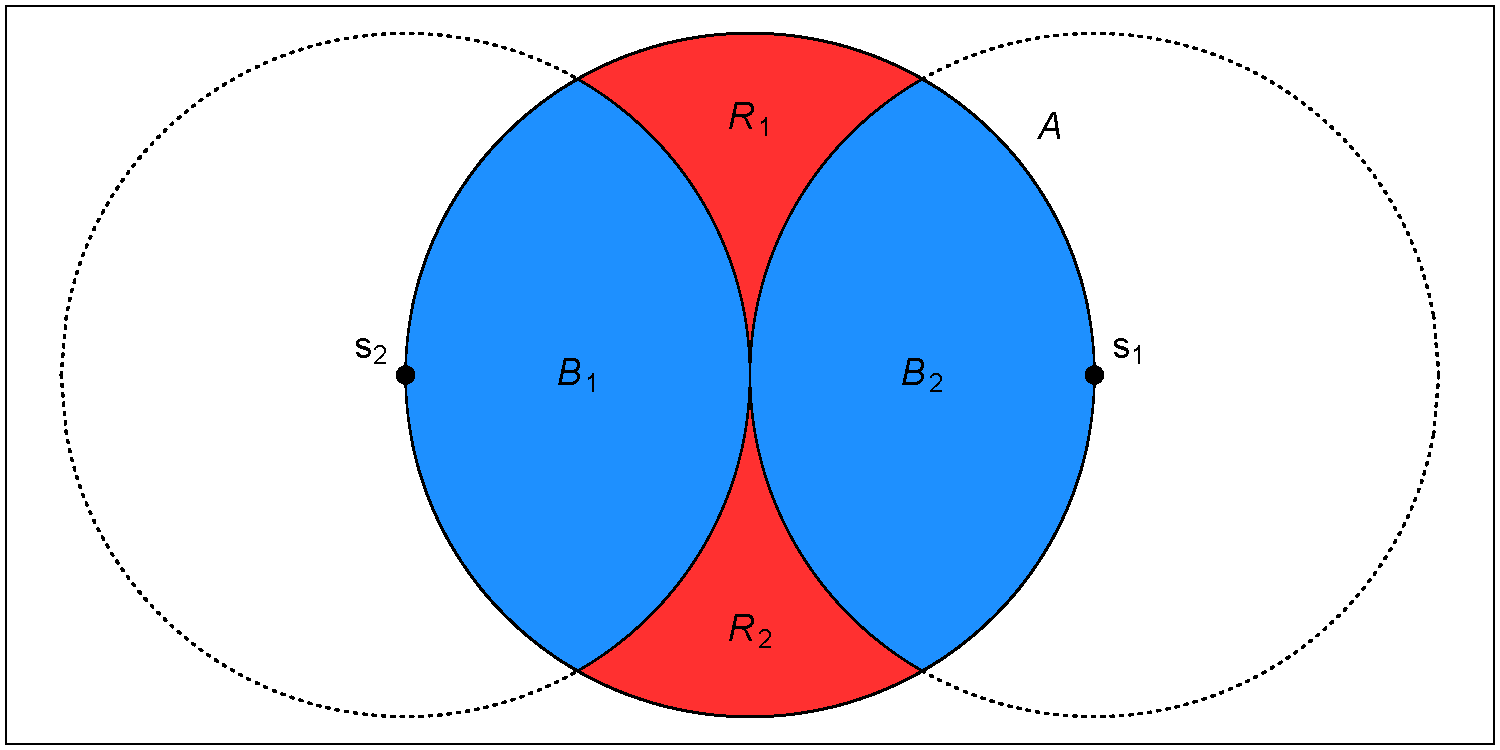
\includegraphics[width=\linewidth]{plots/circles}
  \caption{\DIFaddFL{Illustration of the partition of $A$.}}
  \label{stfig:hpp}
\end{figure}
\DIFadd{Let $N_i$ be the number of knots in $B_i$ and $L_i = l$ if $\bs_i \in P_l$ for $i = 1, 2$.
Then
}\begin{align}
  \DIFadd{P(L_1 \neq L_2) \ge P(N_1 > 0, N_2 > 0)
}\end{align}
\DIFadd{since knots in both $B_1$ and $B_2$ is sufficient, but not necessary, to ensure that }\DIFaddend $\bs_1$ and $\bs_2$ are in different \DIFdelbegin \DIFdel{partitions almost surely if two or more points are in $A$.
Let $N(A)$ be the number of points in $A$, and let
}\begin{eqnarray*}
  \DIFdel{\mu(A) = \mu |A| = \mu \pi \left(\frac{h}{2}\right)^2 = \lambda h^2.
}\end{eqnarray*}
%DIFAUXCMD
\DIFdel{Then
}\begin{eqnarray*}
  \DIFdel{P}[\DIFdel{N(A) \ge 2}] &\DIFdel{= 1 - P}[\DIFdel{N(A) = 0}] \DIFdel{- P}[\DIFdel{N(A) = 1}]\\
                &\DIFdel{= 1 - \exp\{-\lambda h^2\} - \lambda h^2 \exp\{-\lambda h^2\} }\\
                &\DIFdel{= 1 - (1 + \lambda h^2) \exp\{-\lambda h^2\}
}\end{eqnarray*}
%DIFAUXCMD
\DIFdelend \DIFaddbegin \DIFadd{partition sets.
By definition of a Poission process, $N_1$ and $N_2$ are independent and thus $P(N_1 > 0, N_2 > 0) = P(N_1 > 0)^2$, and the intensity measure over $B_1$ is given by
}\begin{align}
  \DIFadd{\mu_{PP}(B_1) }&\DIFadd{= \lambda_{PP} |B_1| = \lambda_{PP} \frac{h^2}{4} \left(\frac{2 \pi}{3} - \frac{\sqrt{3}}{2} \right) \nonumber }\\
       &\DIFadd{= \lambda^*_{PPB1} h^2.
}\end{align}
\DIFadd{So,
}\begin{align}
  \DIFadd{P(L_1 \neq L_2) >= P(N_1 > 0)^2 = }[\DIFadd{1 - P(N_1 = 0)}]\DIFadd{^2 = }[\DIFadd{1 - \exp\left(-\lambda^*_{PPB1} h^2\right)}]\DIFadd{^2
}\end{align}
\DIFaddend which goes to \DIFdelbegin \DIFdel{one as $h \rightarrow \infty$}\DIFdelend \DIFaddbegin \DIFadd{1 as $h$ goes to infinity}\DIFaddend .

%DIF > Then $\bs_1$ and $\bs_2$ are in different partitions almost surely if two or more points are in $A$.
%DIF > Let $N(A)$ be the number of points in $A$, and let
%DIF > \begin{align*}
%DIF >   \mu(A) = \lambda_{PP} |A| = \lambda_{PP} \pi \left(\frac{h}{2}\right)^2 = \lambda_{PP}^* h^2.
%DIF > \end{align*}
\DIFaddbegin 

%DIF > 
%DIF > 
%DIF > Then
%DIF > \begin{align*}
%DIF >   P[N(A) \ge 2] &= 1 - P[N(A) = 0] - P[N(A) = 1]\\
%DIF >                 &= 1 - \exp\{-\lambda h^2\} - \lambda h^2 \exp\{-\lambda h^2\} \\
%DIF >                 &= 1 - (1 + \lambda h^2) \exp\{-\lambda h^2\}
%DIF > \end{align*}
%DIF > which goes to one as $h \rightarrow \infty$.


\DIFaddend % Let $N(A)$ be the number of knots in $A$.
% So,
% \begin{align*}
%   P[ N(A) = k] = \frac{ \mu(A)^k \exp\{ -\mu(A)\}}{k!}.
% \end{align*}
% Then for any finite $k$, $\lim_{h \rightarrow \infty} P[N(A) = k] = 0$ because $\lim_{h \rightarrow \infty} \mu(A) = \infty$.
% With each additional knot in $A$, the chance that $\bs_1$ and $\bs_2$ will be be in the same partition will decrease, because partition membership is defined by the closest knot to a site.
% Therefore, $\lim_{h \rightarrow \infty} \pi(h) = 0$.

% \subsection{Half-normal distribution}
% Let $u = |z|$ where $Z \sim N(\mu, \sigma^2)$.
% Specifically, we consider the case where $\mu = 0$. Then $U$ follows a half-normal distribution which we denote as $U \sim HN(0, 1)$, and the density is given by
% \begin{align}
%   f_U(u) = \frac{ \sqrt{2} }{ \sqrt{\pi \sigma^2} } \exp \left( - \frac{ u^2 }{ 2 \sigma^2 } \right) I(u > 0)
% \end{align}
% When $\mu = 0$, the half-normal distribution is also equivalent to a $N_{(0, \infty)}(0, \sigma^2)$ where $N_{(a, b)}(\mu, \sigma^2)$ represents a normal distribution with mean $\mu$ and standard deviation $\sigma$ that has been truncated below at $a$ and above at $b$.

\section{Skew-$t$ distribution} \DIFdelbegin %DIFDELCMD < %DIFDELCMD < \label{a:skewt}%%%
%DIFDELCMD < %%%
\DIFdelend \DIFaddbegin \label{sta:skewt}
\DIFaddend \subsection*{Univariate skew-$t$ distribution}
We say that $Y$ follows a univariate extended skew-$t$ distribution with location $\xi \in \calR$, scale $\omega > 0$, skew parameter $\alpha \in \calR$, and degrees of freedom $\nu$ if has distribution function
\begin{align}
  f_{\text{EST}}(y) = 2 f_T (z; \nu) F_T\left[ \alpha z \sqrt{ \frac{ \nu + 1 }{ \nu + z^2}}; \nu + 1 \right]
\end{align}
where $f_T(t; \nu)$ is a univariate Student's $t$ with $\nu$ degrees of freedom, $F_T(t; \nu) = P(T < t)$, and \hbox{$z = (y - \xi) / \omega$}.

\subsection*{Multivariate skew-$t$ distribution}
If $\bZ \sim \text{ST}_d(0, \bar{\bOmega}, \balpha, \eta)$ is a $d$-dimensional skew-$t$ distribution, and $\bY = \xi + \bomega \bZ$, where $\bomega = \text{diag}(\omega_1, \ldots, \omega_d)$, then the density of $Y$ at $y$ is
\begin{align}
  f_y(\by) = det(\bomega)^{-1} f_z(\bz)
\end{align}
where
\begin{align}
  f_z(\bz) &= 2 t_d(\bz; \bar{\bOmega}, \eta) T \left[ \balpha\DIFdelbegin \DIFdel{^T }\DIFdelend \DIFaddbegin \DIFadd{^\top }\DIFaddend \bz \sqrt{ \frac{\eta + d}{\nu + Q(\bz)} }; \eta + d\right] \\
  \bz &= \bomega^{-1}(\by - \xi)
\end{align}
where $t_d(\bz; \bar{\bOmega}, \eta)$ is a $d$-dimensional Student's $t$-distribution with scale matrix $\bar{\bOmega}$ and degrees of freedom $\eta$, \DIFdelbegin \DIFdel{$Q(z) = \bz^T \bar{\Omega}^{-1}\bz$ }\DIFdelend \DIFaddbegin \DIFadd{$Q(z) = \bz^\top \bar{\Omega}^{-1}\bz$ }\DIFaddend and $T(\cdot; \eta)$ denotes the univariate Student's $t$ distribution function with $\eta$ degrees of freedom \citep{Azzalini2014}.

\subsection*{Extremal dependence}
For a bivariate skew-$t$ random variable \DIFdelbegin \DIFdel{$\bY = [Y(\bs), Y(\bt)]^T$}\DIFdelend \DIFaddbegin \DIFadd{$\bY = [Y(\bs), Y(\bt)]^\top$}\DIFaddend , the $\chi(h)$ statistic \citep{Padoan2011} is given by
\begin{align} \DIFdelbegin %DIFDELCMD < %DIFDELCMD < \label{eq:chiskew-t}%%%
%DIFDELCMD <   %%%
\DIFdelend \DIFaddbegin \label{steq:chiskew-t}
  \DIFaddend \chi(h) = \bar{F}_{\text{EST}}\left\{ \frac{[x_1^{1 / \eta} - \varrho(h)] \sqrt{\eta + 1} }{\sqrt{1 - \varrho(h)^2}}; 0, 1, \alpha_1, \tau_1, \eta + 1 \right\} + \bar{F}_{\text{EST}}\left\{ \frac{ [x_2^{1 / \eta} - \varrho(h)] \sqrt{\eta + 1} }{ \sqrt{1 - \varrho(h)^2} }; 0, 1, \alpha_2, \tau_2, \eta + 1 \right\},
\end{align}
where $\bar{F}_{\text{EST}}$ is the univariate survival extended skew-$t$ function with zero location and unit scale, \hbox{$\varrho(h) = \text{cor}[y(\bs), y(\bt)]$}, $\alpha_j = \alpha_i \sqrt{1 - \varrho^2}$, $\tau_j = \sqrt{\eta + 1}(\alpha_j + \alpha_i \varrho)$, and $x_j = F_T(\bar{\alpha}_i \sqrt{\eta + 1}; 0, 1, \eta) / F_T(\bar{\alpha}_j \sqrt{\eta + 1}; 0, 1, \eta)$ with $j = 1, 2$ and $i = 2, 1$ and where $\bar{\alpha}_j = (\alpha_j + \alpha_i \varrho) / \sqrt{ 1 + \alpha_i^2 [1 - \varrho(h)^2]}$.

\subsection*{Proof that $\lim_{h \rightarrow \infty} \chi(h) > 0$}
Consider the bivariate distribution of \DIFdelbegin \DIFdel{$\bY = [Y(\bs), Y(\bt)]^T$}\DIFdelend \DIFaddbegin \DIFadd{$\bY = [Y(\bs), Y(\bt)]^\top$}\DIFaddend , with $\varrho(h)$ given by \DIFdelbegin \DIFdel{(\ref{eq:matern})}\DIFdelend \DIFaddbegin \eref{steq:matern}\DIFaddend .
So, $\lim_{h \rightarrow \infty} \varrho(h) = 0$.
Then
\begin{align}
  \lim_{h \rightarrow \infty} \chi(h) = \bar{F}_{\text{EST}}\left\{ \sqrt{\eta + 1}; 0, 1, \alpha_1, \tau_1, \eta + 1 \right\} + \bar{F}_{\text{EST}}\left\{ \sqrt{\eta + 1}; 0, 1, \alpha_2, \tau_2, \eta + 1 \right\}.
\end{align}
Because the extended skew-$t$ distribution is not bounded above, for all $\bar{F}_{\text{EST}}(x) = 1 - F_{\text{EST} (x)} > 0$ for all $x < \infty$.
Therefore, for a skew-$t$ distribution, $\lim_{h \rightarrow \infty} \chi(h) > 0$.

\DIFaddbegin \section{\DIFadd{Comparisons with other parameterizations}} \label{sta:otherparams}
\DIFadd{Various forms of multivariate skew-normal and skew-$t$ distributions have been proposed in the literature.
In this section, we make a connection between our parameterization in }\eref{steq:fullmodel} \DIFadd{of the main text and another popular version.
\mbox{%DIFAUXCMD
\citet{Azzalini2014} }%DIFAUXCMD
and \mbox{%DIFAUXCMD
\citet{Beranger2016} }%DIFAUXCMD
define a skew-normal process as
}\begin{align}
  \DIFadd{\tilde{X}(\bs) = \tilde{\lambda}|z| + (1 - \tilde{\lambda}^2)^{1 / 2} v(\bs)
}\end{align}
\DIFadd{where $\tilde{\lambda} \in (-1, 1)$, $z \sim N(0, 1)$, and $v(\bs)$ is a Gaussian process with mean zero, variance one, and spatial correlation function $\rho$.
To extend this to the skew-$t$ distribution, \mbox{%DIFAUXCMD
\citet{Azzalini2003} }%DIFAUXCMD
take $\tilde{Y}(\bs) = W\tilde{X}(\bs)$ where $W^{-2} \sim $ Gamma$(a / 2, a / 2)$.
Returning to the proposed parameterization (with $\bbeta = 0$), let $W^{-2} = \frac{b}{a}\sigma^{-2} \sim$ Gamma$(a / 2, a / 2)$ so that }\eref{steq:fullmodel} \DIFadd{in the manuscript becomes
}\begin{align}
  \DIFadd{Y(\bs) = W \left[ \lambda \left(\frac{b}{a}\right)^{1 / 2} |z| + \left(\frac{b}{a}\right)^{1 / 2} v(\bs) \right].
}\end{align}
\DIFadd{Clearly setting $b = a (1 - \tilde{\lambda}^2) > 0$, and $\lambda = \tilde{\lambda} / (1 - \tilde{\lambda}^2)^{1 / 2} \in (-\infty, \infty)$ resolves the difference in parameterizations.
We note that our parameterization has three parameters $(a, b, \lambda)$ compared to the two parameters of the alternative parameterization $(a, \tilde{\lambda})$.
Since we have assumed that both $v(\bs)$ and $z$ have unit scale, the additional $b$ parameter in our parameterization is required to control the precision.
%DIF >  However, if we introduce an overall scale parameter $c > 0$ into the alternative parameterization so that $\tilde{Y}(\bs) = c W \tilde{X}(\bs)$, then the two models remain equivalent by setting $a = \nu$, $b = \frac{\nu}{c^2 (1 - \tilde{\lambda}^2)}$, and $\lambda = \tilde{\lambda} / (1 - \tilde{\lambda}^2)^{1 / 2}$.
}

\section{\DIFadd{Temporal dependence}} \label{sta:temporal}
\DIFadd{It is very challenging to derive an analytical expression the temporal extremal dependence at a single site $\bs$.
However, using simulated data, we have evidence to suggest that the model does exhibits temporal extremal dependence.
To demonstrate that our model maintains temporal extremal dependence, we generate lag-$m$ observations for $m = 1, 3, 5, 10$ from our model setting $\phi_w = \phi_z = \phi_\sigma = \varphi$, for $\varphi = 0, 0.02, 0.04, \ldots, 1$.
To estimate the lag-$m$ chi-statistic $\chi(m)$ we first estimate the lag-$m$ $F$-madogram $\nu_F(m)$ \mbox{%DIFAUXCMD
\citep{Cooley2006} }%DIFAUXCMD
using $\hat{\nu}_F(m) = \frac{1}{2n} \sum_{i = 1}^n | \hat{F}(y_{0}) - \hat{F}(y_{m})|$ where $\hat{F}(\cdot)$ represents an empirical CDF and $y_m$ is the lag-$m$ observation.
The $F$-madogram is related to the $\chi$ statistic as follows
}\begin{align}
  \DIFadd{\chi = 2 - \frac{1 + 2 \nu_F}{1 - 2 \nu_F}.
}\end{align}
\DIFadd{\fref{stfig:chiphi} suggests that the extremal dependence increases as $\phi \rightarrow 1$, and that the extremal dependence decreases as $m$ increases.
}\begin{figure}
  \centering
  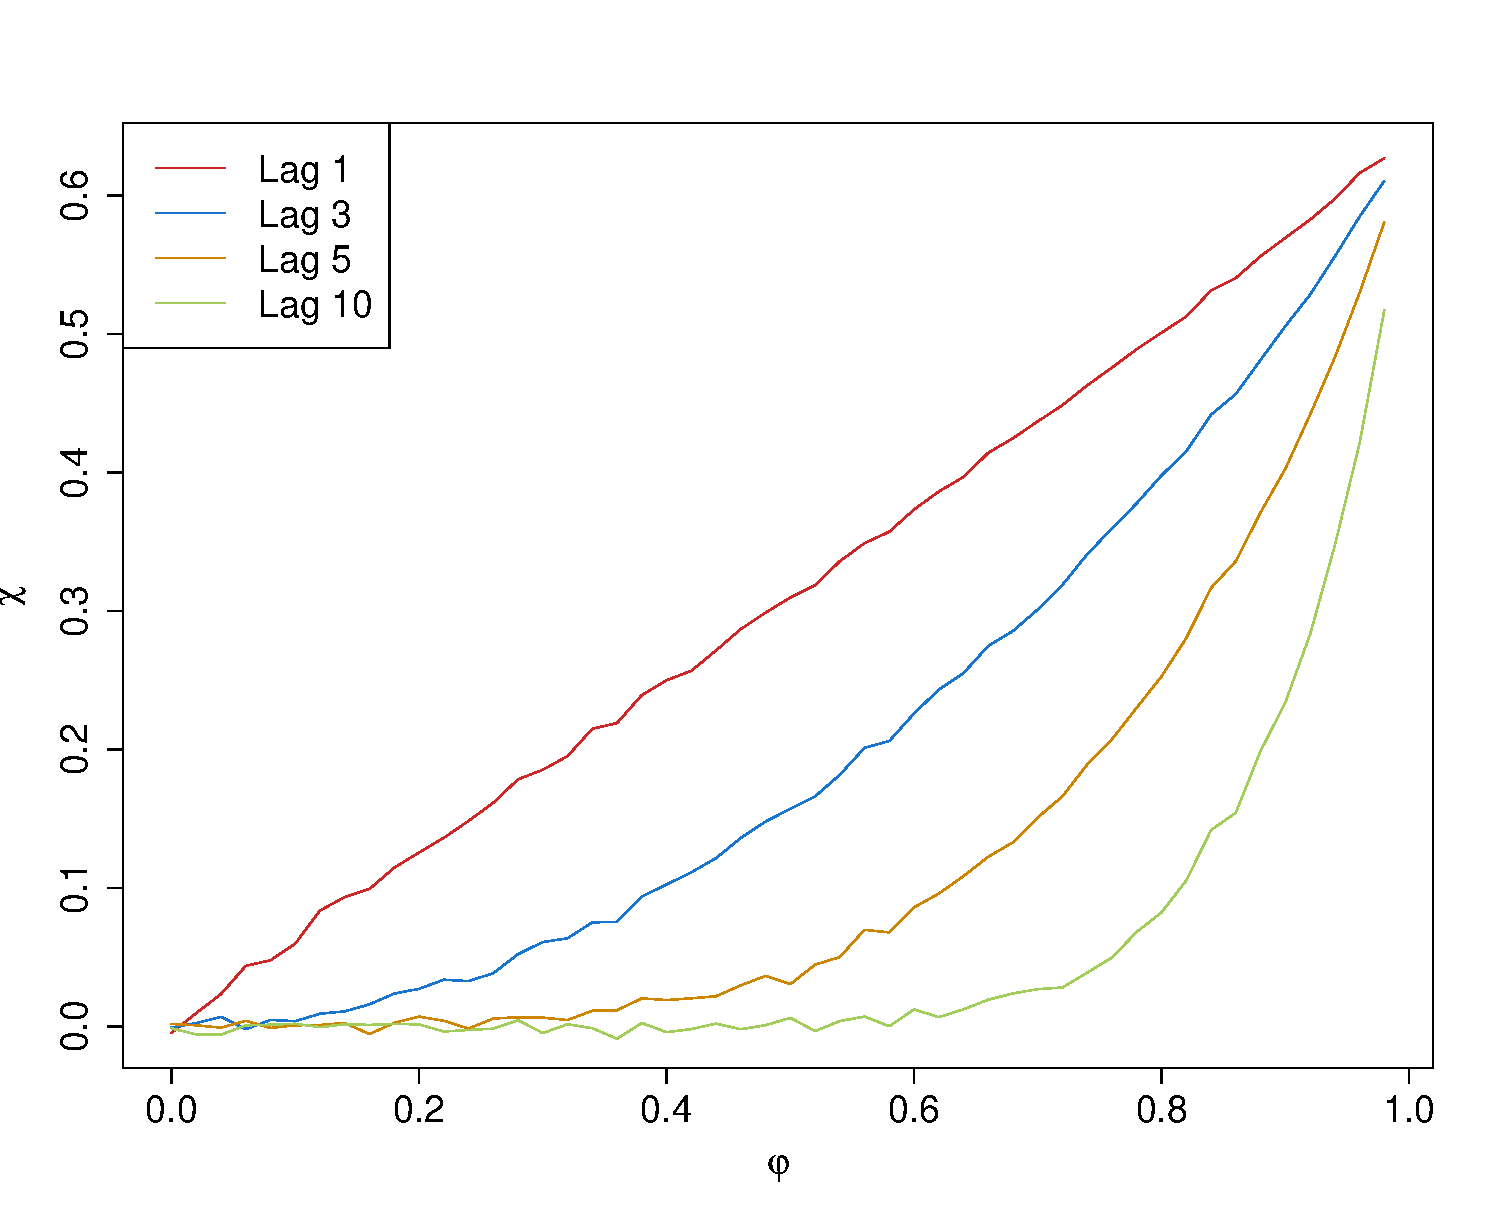
\includegraphics[width=\linewidth]{plots/chi-phi}
  \caption{\DIFaddFL{Simulated lag-$m$ $\chi$ for varying levels of $\varphi$.}}
  \label{stfig:chiphi}
\end{figure}

\section{\DIFadd{Brier scores for ozone prediction}} \label{sta:ozonesite}
\DIFadd{Because typical ozone concentration varies throughout the US, we have included Brier scores by site for two model fits (Gaussian and Skew-$t$, $K = 5$, $T = 50$) in \fref{stfig:bssite}.
As we can see in these plots, both models seem to perform similarly across the US with the poorest performance in California.
Other methods have similar Brier score maps to these.
}\begin{figure}
  \centering
  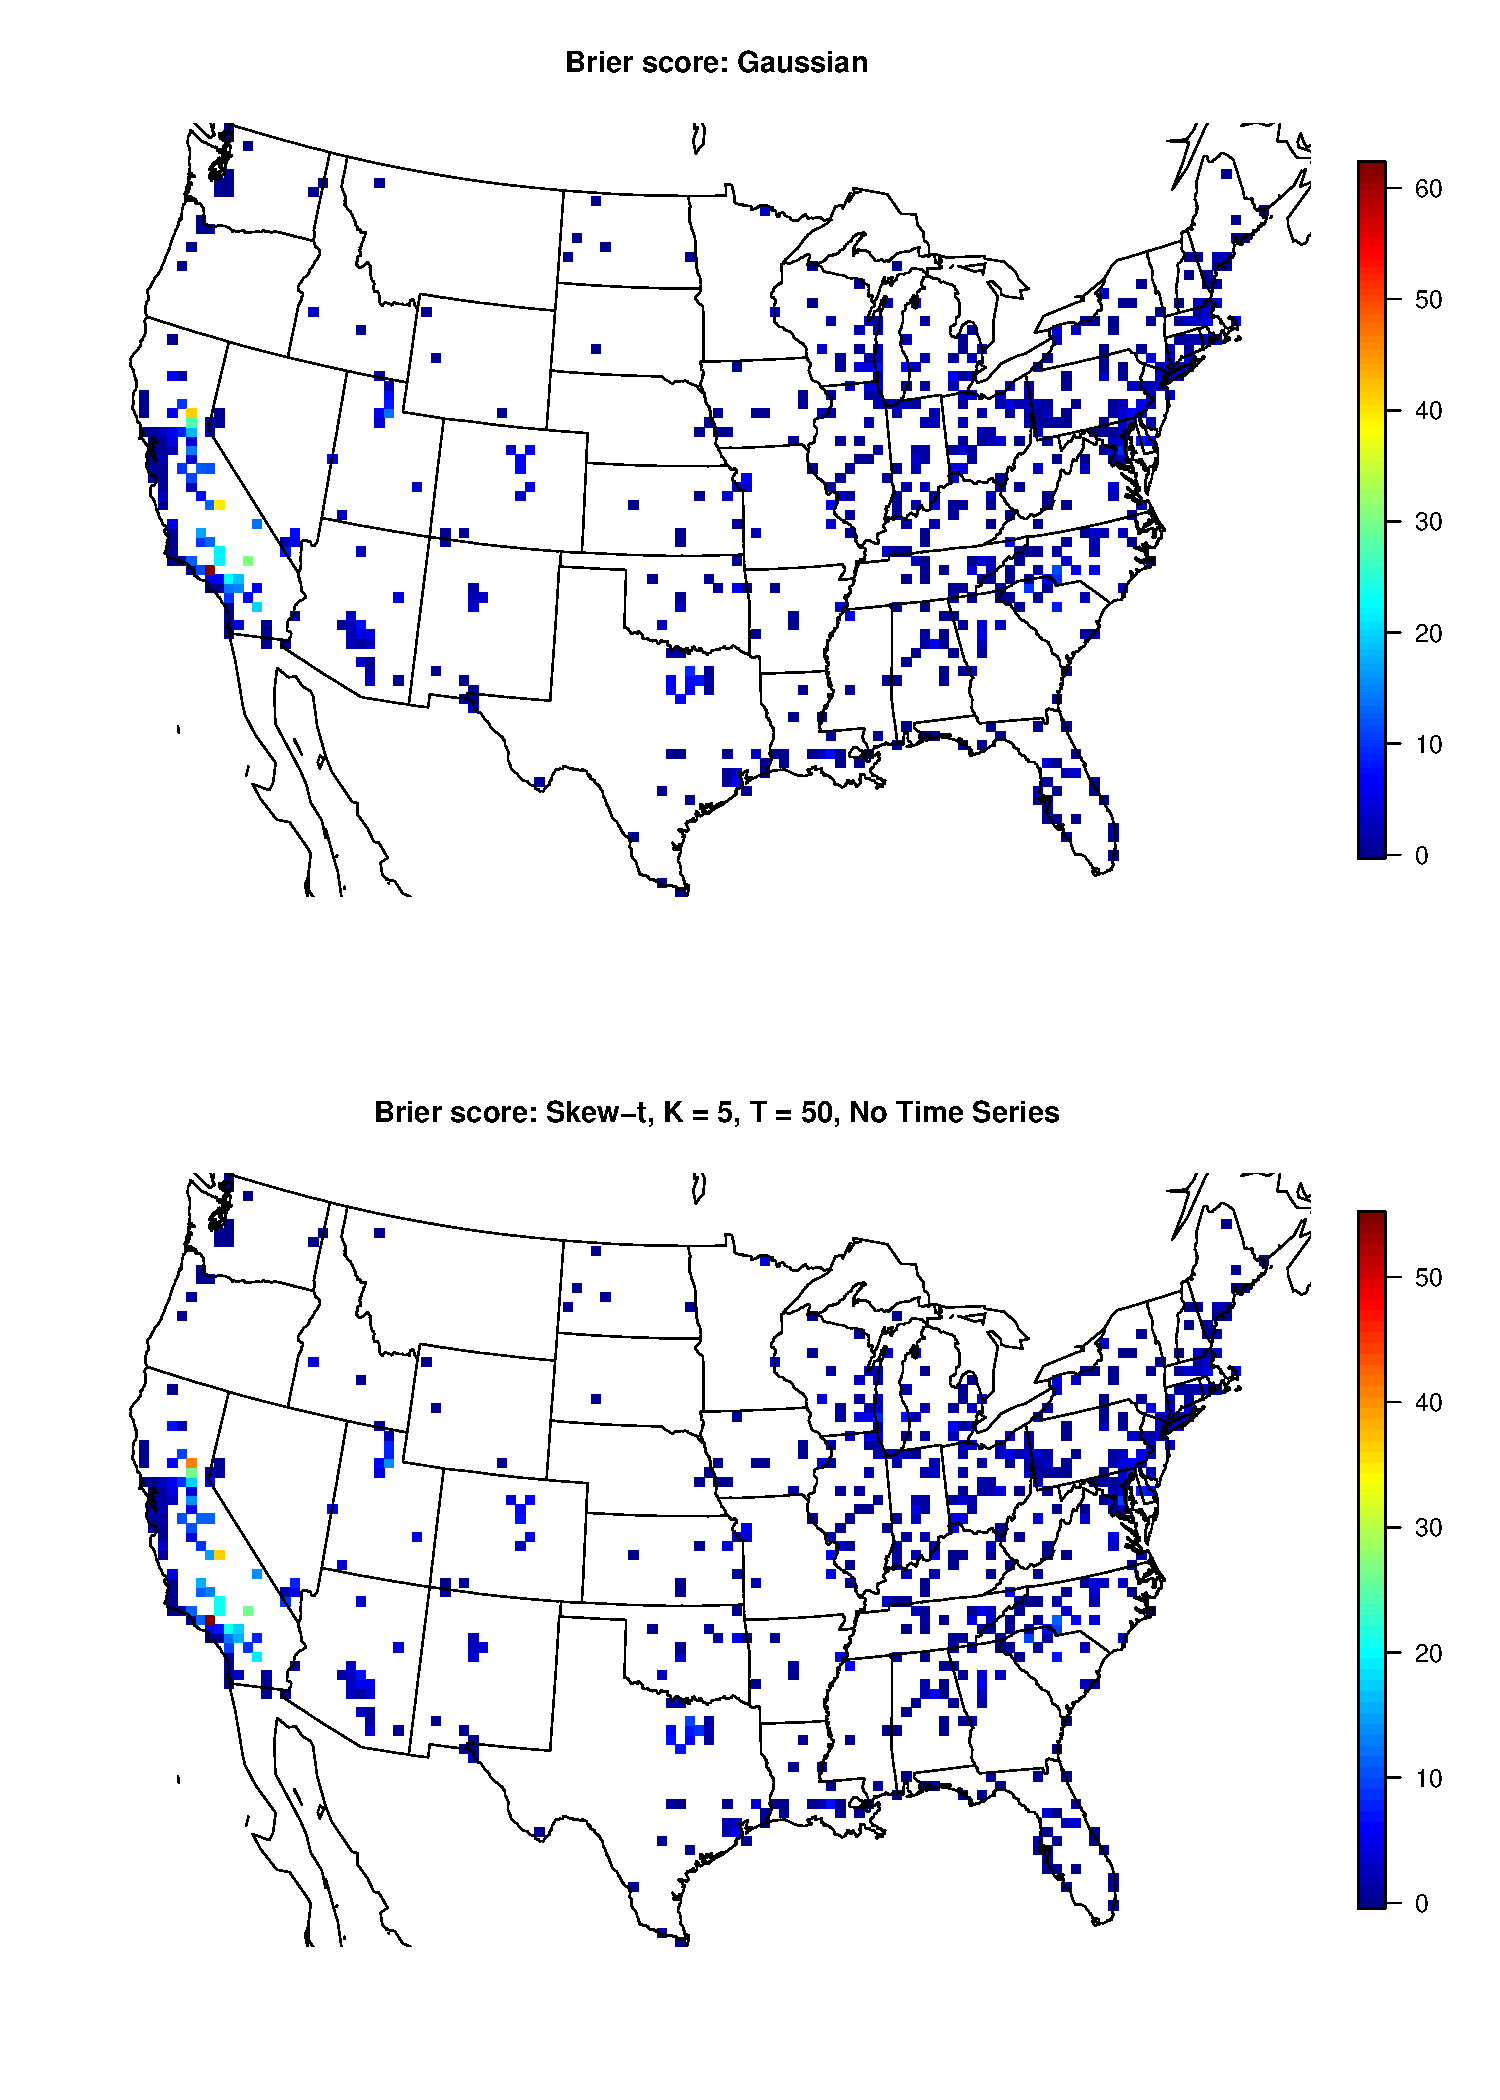
\includegraphics[width=0.8\linewidth]{plots/bs-site}
  \caption{\DIFaddFL{Map of Brier scores for Gaussian (top) vs Skew-$t$, $K = 5$, $T = 50$ (bottom).}}
  \label{stfig:bssite}
\end{figure}

\DIFaddend \section{Simulation study pairwise difference results} \DIFdelbegin %DIFDELCMD < %DIFDELCMD < \label{a:pdiffs}%%%
%DIFDELCMD < %%%
\DIFdelend \DIFaddbegin \label{sta:pdiffs}
\DIFaddend The following tables show the methods that have significantly different Brier scores when using a Wilcoxon-Nemenyi-McDonald-Thompson test.
In each column, different letters signify that the methods have significantly different Brier scores.
For example, there is significant evidence to suggest that method 1 and method 4 have different Brier scores at $q(0.90)$, whereas there is not significant evidence to suggest that method 1 and method 2 have different Brier scores at $q(0.90)$.
In each table group A represents the group with the lowest Brier scores.
Groups are significant with a familywise error rate of $\alpha = 0.05$.

\begin{table}[htbp]
  \centering
  \caption{Setting 1 -- Gaussian marginal, $K = 1$ knot}
  \DIFdelbeginFL %DIFDELCMD < %DIFDELCMD < \label{tbl:gaussim}%%%
%DIFDELCMD <   \begin{tabular}{|l|ccc|ccc|cccc|ccc|}
%DIFDELCMD <     \cline{2-14}
%DIFDELCMD <     %%%
\DIFdelendFL \DIFaddbeginFL \label{sttbl:gaussim}
  \begin{tabular}{|l|ccc|ccc|cccc|cc|}
    \cline{2-13}
    \DIFaddendFL \multicolumn{1}{c}{} & \multicolumn{3}{|c}{$q(0.90)$} & \multicolumn{3}{|c}{$q(0.95)$} & \multicolumn{4}{|c}{$q(0.98)$} & \DIFdelbeginFL %DIFDELCMD < \multicolumn{3}{|c|}{$q(0.99)$} %%%
\DIFdelendFL \DIFaddbeginFL \multicolumn{2}{|c|}{$q(0.99)$} \DIFaddendFL \\
    \hline
    Method 1 & A &   &   & A &   &   & A &   &   &   & A &   \DIFdelbeginFL \DIFdelFL{B }%DIFDELCMD < &   %%%
\DIFdelendFL \\
    \hline
    Method 2 & A &   &   & A &   &   & A &   &   &   & A &   \DIFdelbeginFL %DIFDELCMD < &   %%%
\DIFdelendFL \\
    \hline
    Method 3 &   & B &   &   & B &   &   &   & C &   & \DIFaddbeginFL \DIFaddFL{A }\DIFaddendFL &   \DIFdelbeginFL \DIFdelFL{B }%DIFDELCMD < &   %%%
\DIFdelendFL \\
    \hline
    Method 4 & A &   &   & A &   &   & A & B &   &   & A &   \DIFdelbeginFL \DIFdelFL{B }%DIFDELCMD < &   %%%
\DIFdelendFL \\
    \hline
    Method 5 &   & B &   &   & B &   &   & B & C &   & A &   \DIFdelbeginFL \DIFdelFL{B }%DIFDELCMD < &   %%%
\DIFdelendFL \\
    \hline
    Method 6 &   &   & C &   &   & C &   &   &   & D &   & \DIFdelbeginFL %DIFDELCMD < & %%%
\DIFdelFL{C }\DIFdelendFL \DIFaddbeginFL \DIFaddFL{B }\DIFaddendFL \\
    \hline
  \end{tabular}
\end{table}

% \begin{table}[htbp]
%   \centering
%   \caption{Setting 2: Symmetric-$t$ marginal, $K = 1$ knot}
%   \label{tbl:t1k1sim}
%   \begin{tabular}{|l|cc|cccc|cccc|ccc|}
%     \cline{2-14}
%     \multicolumn{1}{c}{} & \multicolumn{2}{|c}{$q(0.90)$} & \multicolumn{4}{|c}{$q(0.95)$} & \multicolumn{4}{|c}{$q(0.98)$} & \multicolumn{3}{|c|}{$q(0.99)$} \\
%     \hline
%     Method 1 &   & B &   &   &   & D &   &   &   & D &   &   & C \\
%     \hline
%     Method 2 & A &   & A &   &   &   & A &   &   &   & A &   &   \\
%     \hline
%     Method 3 &   & B &   & B &   &   &   & B & C &   &   & B &   \\
%     \hline
%     Method 4 & A &   &   &   & C &   &   & B &   &   &   & B &   \\
%     \hline
%     Method 5 &   & B &   &   &   & D &   &   & C & D &   & B & C \\
%     \hline
%   \end{tabular}
% \end{table}

% \begin{table}[htbp]
%   \centering
%   \caption{Setting 3: Symmetric-$t$ marginal, $K = 5$ knots}
%   \label{tbl:gaussim}
%   \begin{tabular}{|l|cc|cc|cc|cc|}
%     \cline{2-9}
%     \multicolumn{1}{c}{} & \multicolumn{2}{|c}{$q(0.90)$} & \multicolumn{2}{|c}{$q(0.95)$} & \multicolumn{2}{|c}{$q(0.98)$} & \multicolumn{2}{|c|}{$q(0.99)$} \\
%     \hline
%     Method 1 &   & B &   & B &   & B &   & B \\
%     \hline
%     Method 2 &   & B &   & B &   & B &   & B \\
%     \hline
%     Method 3 &   & B &   & B &   & B & A & B \\
%     \hline
%     Method 4 & A &   & A &   & A &   & A &   \\
%     \hline
%     Method 5 &   & B &   & B & A & B & A & B \\
%     \hline
%   \end{tabular}
% \end{table}

\begin{table}[htbp]
  \centering
  \caption{Setting 2 -- Skew-$t$ marginal, $K = 1$ knot}
  \DIFdelbeginFL %DIFDELCMD < %DIFDELCMD < \label{tbl:st1sim}%%%
%DIFDELCMD <   \begin{tabular}{|l|ccccc|cccc|cccc|ccc|}
%DIFDELCMD <     \cline{2-17}
%DIFDELCMD <     %%%
\DIFdelendFL \DIFaddbeginFL \label{sttbl:st1sim}
  \begin{tabular}{|l|cccc|cccc|cccc|ccc|}
    \cline{2-16}
    \DIFaddendFL \multicolumn{1}{c}{} & \DIFdelbeginFL %DIFDELCMD < \multicolumn{5}{|c}{$q(0.90)$} %%%
\DIFdelendFL \DIFaddbeginFL \multicolumn{4}{|c}{$q(0.90)$} \DIFaddendFL & \multicolumn{4}{|c}{$q(0.95)$} & \multicolumn{4}{|c}{$q(0.98)$} & \multicolumn{3}{|c|}{$q(0.99)$} \\
    \hline
    Method 1 &   & \DIFaddbeginFL \DIFaddFL{B }\DIFaddendFL &   \DIFdelbeginFL \DIFdelFL{C }\DIFdelendFL &   &   & \DIFdelbeginFL %DIFDELCMD < & %%%
\DIFdelendFL B &   &   &   & B &   \DIFdelbeginFL \DIFdelFL{C }\DIFdelendFL &   &   & B &   \\
    \hline
    Method 2 & A &   &   &   & \DIFdelbeginFL %DIFDELCMD < & %%%
\DIFdelendFL A &   &   &   & A &   &   &   & A &   &   \\
    \hline
    Method 3 & \DIFaddbeginFL \DIFaddFL{A }\DIFaddendFL & B &   \DIFdelbeginFL \DIFdelFL{C }\DIFdelendFL &   & \DIFdelbeginFL %DIFDELCMD < & %%%
\DIFdelendFL A & B &   &   & A & B &   &   & A & B &   \\
    \hline
    Method 4 & A & B &   &   & \DIFaddbeginFL \DIFaddFL{A }\DIFaddendFL & \DIFdelbeginFL %DIFDELCMD < & %%%
\DIFdelendFL B &   &   & \DIFaddbeginFL \DIFaddFL{A }\DIFaddendFL & B &   &   & A & \DIFaddbeginFL \DIFaddFL{B }\DIFaddendFL &   \\
    \hline
    Method 5 &   &   & \DIFaddbeginFL \DIFaddFL{C }\DIFaddendFL &   \DIFdelbeginFL \DIFdelFL{D }\DIFdelendFL &   &   & \DIFdelbeginFL %DIFDELCMD < & %%%
\DIFdelendFL C &   &   &   & C &   &   &   \DIFdelbeginFL \DIFdelFL{B }\DIFdelendFL & \DIFaddbeginFL \DIFaddFL{C }\DIFaddendFL \\
    \hline
    Method 6 &   &   &   & \DIFaddbeginFL \DIFaddFL{D }\DIFaddendFL &   \DIFdelbeginFL \DIFdelFL{E }\DIFdelendFL &   &   & \DIFdelbeginFL %DIFDELCMD < & %%%
\DIFdelendFL D &   &   &   & D &   &   & C \\
    \hline
  \end{tabular}
\end{table}

\begin{table}[htbp]
  \centering
  \caption{Setting 3 -- Skew-$t$ marginal, $K = 5$ knots}
  \DIFdelbeginFL %DIFDELCMD < %DIFDELCMD < \label{tbl:st5sim}%%%
%DIFDELCMD <   \begin{tabular}{|l|ccc|cccc|ccc|ccc|}
%DIFDELCMD <     \cline{2-14}
%DIFDELCMD <     %%%
\DIFdelendFL \DIFaddbeginFL \label{sttbl:st5sim}
  \begin{tabular}{|l|cccc|cccc|ccc|ccc|}
    \cline{2-15}
    \DIFaddendFL \multicolumn{1}{c}{} & \DIFdelbeginFL %DIFDELCMD < \multicolumn{3}{|c}{$q(0.90)$} %%%
\DIFdelendFL \DIFaddbeginFL \multicolumn{4}{|c}{$q(0.90)$} \DIFaddendFL & \multicolumn{4}{|c}{$q(0.95)$} & \multicolumn{3}{|c}{$q(0.98)$} & \multicolumn{3}{|c|}{$q(0.99)$} \\
    \hline
    Method 1 &   &   \DIFdelbeginFL \DIFdelFL{B }\DIFdelendFL & \DIFaddbeginFL \DIFaddFL{C }\DIFaddendFL &   &   &   \DIFaddbeginFL & \DIFaddendFL C &   &   & B &   &   & B &   \\
    \hline
    Method 2 &   &   \DIFdelbeginFL \DIFdelFL{B }\DIFdelendFL & \DIFaddbeginFL \DIFaddFL{C }\DIFaddendFL &   &   &   \DIFaddbeginFL & \DIFaddendFL C &   &   & B &   &   & B &   \\
    \hline
    Method 3 &   \DIFdelbeginFL \DIFdelFL{A }\DIFdelendFL & \DIFaddbeginFL \DIFaddFL{B }\DIFaddendFL &   &   &   \DIFaddbeginFL & \DIFaddendFL B &   &   & \DIFaddbeginFL \DIFaddFL{A }\DIFaddendFL &   \DIFdelbeginFL \DIFdelFL{B }\DIFdelendFL &   & \DIFaddbeginFL \DIFaddFL{A }\DIFaddendFL &   \DIFdelbeginFL \DIFdelFL{B }\DIFdelendFL &   \\
    \hline
    Method 4 & A &   &   &   \DIFaddbeginFL & \DIFaddendFL A &   &   &   & A &   &   & A &   &   \\
    \hline
    Method 5 & A &   &   &   \DIFaddbeginFL & \DIFaddendFL A &   &   &   & A &   &   & A &   &   \\
    \hline
    Method 6 &   &   &   \DIFdelbeginFL \DIFdelFL{C }\DIFdelendFL & \DIFaddbeginFL \DIFaddFL{D }\DIFaddendFL &   &   &   \DIFaddbeginFL & \DIFaddendFL D &   &   & C &   &   & C \\
    \hline
  \end{tabular}
\end{table}

\begin{table}[htbp]
  \centering
  \caption{Setting 4 -- Max-stable}
  \DIFdelbeginFL %DIFDELCMD < %DIFDELCMD < \label{tbl:mssim}%%%
%DIFDELCMD <   %%%
\DIFdelendFL \DIFaddbeginFL \label{sttbl:mssim}
  \DIFaddendFL \begin{tabular}{|l|cccc|cccc|ccc|ccc|}
    \cline{2-15}
    \multicolumn{1}{c}{} & \multicolumn{4}{|c}{$q(0.90)$} & \multicolumn{4}{|c}{$q(0.95)$} & \multicolumn{3}{|c}{$q(0.98)$} & \multicolumn{3}{|c|}{$q(0.99)$} \\
    \hline
    Method 1 & A & B &   &   &   & B &   &   &   & B &   &   &   & C \\
    \hline
    Method 2 &   & B &   &   &   & B &   \DIFdelbeginFL \DIFdelFL{C }\DIFdelendFL &   &   & B &   &   & B & C \\
    \hline
    Method 3 &   &   & C & D &   &   & C &   &   & B &   &   & B &   \\
    \hline
    Method 4 &   &   &   & D &   &   &   & D &   &   & C &   &   & C \\
    \hline
    Method 5 &   &   & C &   &   & \DIFaddbeginFL \DIFaddFL{B }\DIFaddendFL & C &   &   & B &   &   & B & C \\
    \hline
    Method 6 & A &   &   &   & A &   &   &   & A &   &   & A &   &   \\
    \hline
  \end{tabular}
\end{table}

\begin{table}[htbp]
  \centering
  \caption{Setting 5 -- \DIFdelbeginFL \DIFdelFL{Transformation below $T = q(0.80)$}\DIFdelendFL \DIFaddbeginFL \DIFaddFL{Brown Resnick}\DIFaddendFL }
  \DIFdelbeginFL %DIFDELCMD < %DIFDELCMD < \label{tbl:transsim}%%%
%DIFDELCMD <   \begin{tabular}{|l|cccc|ccc|cccc|cccc|}
%DIFDELCMD <     \cline{2-16}
%DIFDELCMD <     %%%
\DIFdelendFL \DIFaddbeginFL \label{sttbl:transsim}
  \begin{tabular}{|l|cccc|ccc|ccc|ccc|}
    \cline{2-14}
    \DIFaddendFL \multicolumn{1}{c}{} & \multicolumn{4}{|c}{$q(0.90)$} & \multicolumn{3}{|c}{$q(0.95)$} & \DIFdelbeginFL %DIFDELCMD < \multicolumn{4}{|c}{$q(0.98)$} %%%
\DIFdelendFL \DIFaddbeginFL \multicolumn{3}{|c}{$q(0.98)$} \DIFaddendFL & \DIFdelbeginFL %DIFDELCMD < \multicolumn{4}{|c|}{$q(0.99)$} %%%
\DIFdelendFL \DIFaddbeginFL \multicolumn{3}{|c|}{$q(0.99)$} \DIFaddendFL \\
    \hline
    Method 1 &   &   &   \DIFdelbeginFL \DIFdelFL{C }\DIFdelendFL & \DIFaddbeginFL \DIFaddFL{D }\DIFaddendFL &   &   \DIFdelbeginFL \DIFdelFL{B }\DIFdelendFL & \DIFaddbeginFL \DIFaddFL{C }\DIFaddendFL &   &   & C &   &   & \DIFdelbeginFL %DIFDELCMD < & %%%
\DIFdelFL{C }%DIFDELCMD < &   %%%
\DIFdelendFL \DIFaddbeginFL \DIFaddFL{C }\DIFaddendFL \\
    \hline
    Method 2 &   &   \DIFdelbeginFL \DIFdelFL{B }\DIFdelendFL &   & \DIFaddbeginFL \DIFaddFL{D }\DIFaddendFL &   &   \DIFdelbeginFL \DIFdelFL{B }\DIFdelendFL & \DIFaddbeginFL \DIFaddFL{C }\DIFaddendFL &   &   \DIFdelbeginFL \DIFdelFL{B }\DIFdelendFL & \DIFaddbeginFL \DIFaddFL{C }\DIFaddendFL &   &   \DIFdelbeginFL \DIFdelFL{A }\DIFdelendFL & \DIFdelbeginFL \DIFdelFL{B }%DIFDELCMD < &   &   %%%
\DIFdelendFL \DIFaddbeginFL \DIFaddFL{C }\DIFaddendFL \\
    \hline
    Method 3 & A & \DIFaddbeginFL \DIFaddFL{B }\DIFaddendFL &   &   & A &   &   & A & \DIFaddbeginFL \DIFaddFL{B }\DIFaddendFL &   &   & \DIFdelbeginFL \DIFdelFL{A }\DIFdelendFL \DIFaddbeginFL \DIFaddFL{B }\DIFaddendFL &   \DIFdelbeginFL %DIFDELCMD < &   &   %%%
\DIFdelendFL \\
    \hline
    Method 4 &   &   \DIFdelbeginFL \DIFdelFL{B }\DIFdelendFL & C &   &   & B &   &   & B &   &   & \DIFdelbeginFL %DIFDELCMD < & %%%
\DIFdelendFL B &   \DIFdelbeginFL \DIFdelFL{C }%DIFDELCMD < &   %%%
\DIFdelendFL \\
    \hline
    Method 5 & \DIFaddbeginFL \DIFaddFL{A }\DIFaddendFL &   \DIFdelbeginFL \DIFdelFL{B }\DIFdelendFL &   &   & \DIFaddbeginFL \DIFaddFL{A }\DIFaddendFL &   \DIFdelbeginFL \DIFdelFL{B }\DIFdelendFL &   & \DIFaddbeginFL \DIFaddFL{A }\DIFaddendFL &   \DIFdelbeginFL \DIFdelFL{B }\DIFdelendFL &   \DIFdelbeginFL \DIFdelFL{C }\DIFdelendFL & \DIFaddbeginFL \DIFaddFL{A }\DIFaddendFL & \DIFaddbeginFL \DIFaddFL{B }\DIFaddendFL &   \DIFdelbeginFL %DIFDELCMD < & %%%
\DIFdelFL{C }%DIFDELCMD < &   %%%
\DIFdelendFL \\
    \hline
    Method 6 &   & \DIFaddbeginFL \DIFaddFL{B }\DIFaddendFL & \DIFaddbeginFL \DIFaddFL{C }\DIFaddendFL &   \DIFdelbeginFL \DIFdelFL{D }\DIFdelendFL & \DIFaddbeginFL \DIFaddFL{A }\DIFaddendFL &   &   \DIFdelbeginFL \DIFdelFL{C }\DIFdelendFL & \DIFaddbeginFL \DIFaddFL{A }\DIFaddendFL &   &   & \DIFdelbeginFL \DIFdelFL{D }\DIFdelendFL \DIFaddbeginFL \DIFaddFL{A }\DIFaddendFL &   &   \DIFdelbeginFL %DIFDELCMD < &   & %%%
\DIFdelFL{D }\DIFdelendFL \\
    \hline
  \end{tabular}
\end{table}

% \begin{singlespace}
\bibliographystyle{biom}
\bibliography{library}
% \end{singlespace}

\end{document}

